%\title{LaTeX Portrait Poster Template}
%%%%%%%%%%%%%%%%%%%%%%%%%%%%%%%%%%%%%%%%%
% a0poster Portrait Poster
% LaTeX Template
% Version 1.0 (22/06/13)
%
% The a0poster class was created by:
% Gerlinde Kettl and Matthias Weiser (tex@kettl.de)
% 
% This template has been downloaded from:
% http://www.LaTeXTemplates.com
%
% License:
% CC BY-NC-SA 3.0 (http://creativecommons.org/licenses/by-nc-sa/3.0/)
%
%%%%%%%%%%%%%%%%%%%%%%%%%%%%%%%%%%%%%%%%%

%----------------------------------------------------------------------------------------
%	PACKAGES AND OTHER DOCUMENT CONFIGURATIONS
%----------------------------------------------------------------------------------------

\documentclass[a0,portrait]{a0poster}

\usepackage{multicol} % This is so we can have multiple columns of text side-by-side
\columnsep=100pt % This is the amount of white space between the columns in the poster
\columnseprule=3pt % This is the thickness of the black line between the columns in the poster

\usepackage[svgnames]{xcolor} % Specify colors by their 'svgnames', for a full list of all colors available see here: http://www.latextemplates.com/svgnames-colors

\usepackage{times} % Use the times font
%\usepackage{palatino} % Uncomment to use the Palatino font

\usepackage{graphicx} % Required for including images
\graphicspath{{./imgs/} {./}} % Location of the graphics files
\usepackage{booktabs} % Top and bottom rules for table
\usepackage[font=small,labelfont=bf]{caption} % Required for specifying captions to tables and figures
\usepackage{amsfonts, amsmath, amsthm, amssymb} % For math fonts, symbols and environments
\usepackage{wrapfig} % Allows wrapping text around tables and figures

\begin{document}

%----------------------------------------------------------------------------------------
%	POSTER HEADER 
%----------------------------------------------------------------------------------------

% The header is divided into two boxes:
% The first is 75% wide and houses the title, subtitle, names, university/organization and contact information
% The second is 25% wide and houses a logo for your university/organization or a photo of you
% The widths of these boxes can be easily edited to accommodate your content as you see fit

\begin{minipage}[b]{0.78\linewidth}
\Huge \color{NavyBlue} \textbf{Focused Depth-first Proof Number Search using
Convolutional Neural Networks for the Game of
Hex (\#2034)} \color{Black}\\ % Title
%\Huge\textit{Country Update}\\[2.4cm] % Subtitle
\huge \textbf{Chao Gao, Martin M\"{u}ller, Ryan Hayward}\\[0.5cm] % Author(s)
\huge University of Alberta, Department of Computing Science, Canada\\[0.4cm] % University/organization
\Large \texttt{cgao3@ualberta.ca} \\
\end{minipage}
%
\begin{minipage}[b]{0.2\linewidth}
%
\includegraphics[width=7cm]{ua_logo.pdf}\ 

\includegraphics[width=14cm]{ua_logo.pdf}\\
\end{minipage}

\vspace{1cm} % A bit of extra whitespace between the header and poster content

%----------------------------------------------------------------------------------------

\begin{multicols}{3} % This is how many columns your poster will be broken into, a portrait poster is generally split into 2 columns

%----------------------------------------------------------------------------------------
%	ABSTRACT
%----------------------------------------------------------------------------------------

\color{Navy} % Navy color for the abstract

\begin{abstract}
The game of Hex is a two-player, perfect information and zero-sum board games where no draws exist. Solving the game of Hex can be formulated as searching for a solution in an AND/OR graph. Proof Number Search is an effective algorithm for establishing theoretic values on games with non-uniform branching factor. 
We investigate how to use strength Convolutional Neural Networks (CNNs) to improve proof number search. We describe FDFPN-CNN to address the uniform-branching factor problem in Hex. FDFPN-CNN integrates two CNNs trained from games played by expert players. The value approximation CNN provides reliable information for defining the widening size by estimating the value of the expanding nodes, while the policy CNN selects promising children nodes to the search. 
We show that, on $8\times 8$ Hex, FDFPN-CNN performs much better than the original FDFPN.
\end{abstract}
%----------------------------------------------------------------------------------------
%	INTRODUCTION
%----------------------------------------------------------------------------------------

\color{Black} % SaddleBrown color for the introduction
\section*{Game of Hex}

\begin{minipage}{0.5\linewidth}
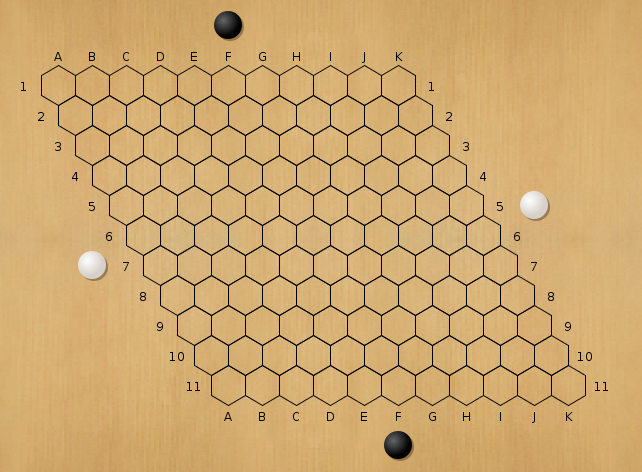
\includegraphics[scale=0.5]{hexboard.png} \\
\end{minipage}
\begin{minipage}{0.5\linewidth}
The game of Hex is invented in 1942 by Piet Hein and in 1948 independently by John Nash. It has been an active domain of artificial intelligence since Shannon's work in 1950s.

The most popular board size is $11\times 11$ (as shown left).
\end{minipage}
Facts we know about Hex:
\begin{itemize}
\item By strategy-stealing argument, there is a winning strategy for first player on initial board position.
\item The explicit strategy is unknown.
\item Solving arbitrary Hex position is PSPACE-Complete.
\end{itemize}

Automatic computer solver requires efficient tree search. 
Solving all openings is of particular interest since Hex is usually played with \emph{swap} rule.

Board sizes solved:
\begin{itemize}
\item $7\times 7$ Hex is solved in 2004 by depth-first search + a number of knowledge pruning. 
\item $8 \times 8$ first solved in 2008 by improved H-search + improved knowledge pruning + depth-first search. In 2011, it is shown that Focused depth-first proof number search is twice faster than DFS.
\item $9 \times 9$ solved in 2014 by parallel FDFPN, took $>$ 17 months. 
\end{itemize}

\color{Black} % DarkSlateGray color for the rest of the content

\section*{Focused depth-first proof number search with CNNs}

Proof/disproof number of a node is the minimum number of leaf nodes that if solved to establish the value of this node. 
\begin{minipage}{0.5\linewidth}
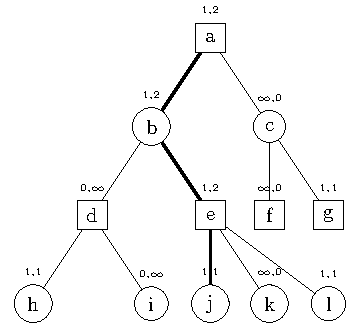
\includegraphics[width=\textwidth]{pns_example.pdf} \\
\end{minipage}
\begin{minipage}{0.4\linewidth}

In trees, those numbers can be calculated from bottom up. 
\begin{itemize}
\item $\phi(s) = \min_{s' \in children(s)} \delta(s')$
\item $\delta(s) = \sum_{s' \in children(s)} \phi(s')$
\end{itemize}
\end{minipage}

$\phi(s)$ and $\delta(s)$ are respectively the minimum number of leaf nodes to prove or disprove $s$. 
Following $\phi, \delta$, there exists most proving node, which potentially would lead to the least effort to solve the root.

\vspace{1cm}
Proof number search works in an iterative fashion: 
\begin{enumerate}
\item Select an Most Proving Node (MPN)
\item Expand MPN, set children's proof and disproof number
\item Backup 
\end{enumerate}

Depth-first proof number search (DFPN) reformulates on PNS, employing bounds to avoid unnecessary traversal in the tree. 
It is more efficient than PNS.

PNS or DFPN does not work well when the game has near uniform branching factor. 
Focused DFPN with CNNs is to address the near-uniform branching factor in Hex. FDFPN-CNN is a redefinition of FDFPN by the following modifications at each expanding node:
\begin{itemize}
\item Resistance for move sorting $\Rightarrow$ A policy net for sorting moves;
\item Fixed widening factor $\mu$ $\Rightarrow$ A value neural net for dynamically choosing a widening factor.
\end{itemize}

\begin{center}\vspace{1cm}
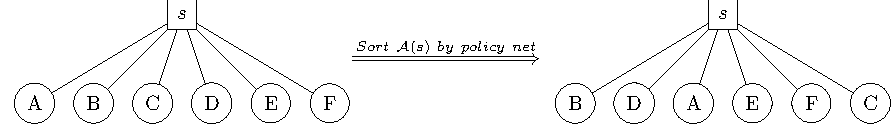
\includegraphics[width=0.8\linewidth]{andor1.pdf}
\captionof{figure}{\color{Green} A policy neural net is used to order the children of an expanding node.}
\end{center}%\vspace{1cm}

\begin{center}\vspace{1cm}
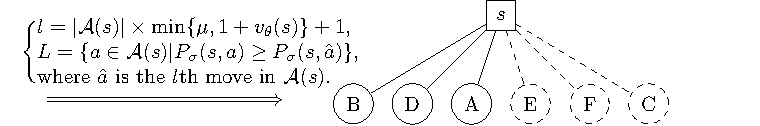
\includegraphics[width=0.8\linewidth]{andor2.pdf}
\captionof{figure}{\color{Green} A value neural net is used to decide window size.}
\end{center}%\vspace{1cm}

The value net helps create an ``artificial'' non-uniform branching factor, making proof number search prefers nodes with small value estimation. 
\begin{center}\vspace{1cm}
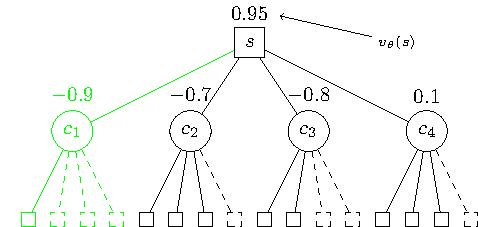
\includegraphics[width=0.7\linewidth]{andor_why_prefer_small_value_net_estimation.pdf}
\captionof{figure}{\color{Green} The smaller value estimation, the smaller expanding window.}
\end{center}%\vspace{1cm}

\section*{Policy and value net}
\textbf{DATA:} $6.5\times 10^5$ state-action or state-value pairs produced by MoHex vs MoHex or MoHex vs Wolve play. 

\subsection*{Architectures}
Input feature planes consist of black, white, empty, black-bridge endpoints, white-bridge endpoints.

\begin{minipage}{0.5\linewidth}\vspace{1cm}
\begin{center}
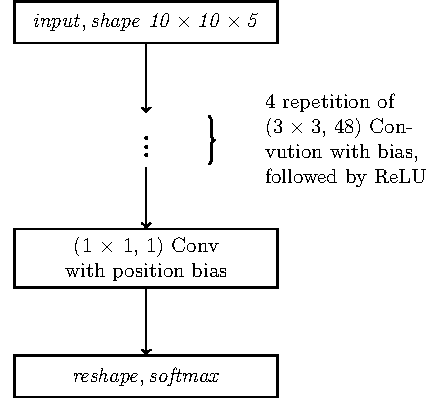
\includegraphics[width=0.9\linewidth]{architecture.pdf}
\captionof{figure}{\color{Green} Policy neural net architecture~~~~}
\end{center}
\end{minipage}\vspace{1cm}
\begin{minipage}{0.5\linewidth}\vspace{1cm}
\begin{center}
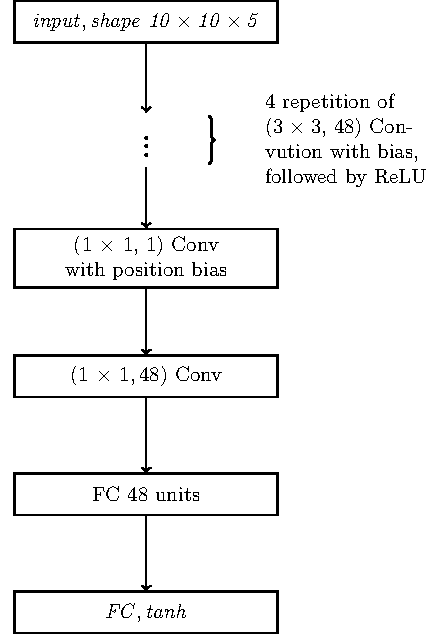
\includegraphics[width=0.55\linewidth]{architec_value.pdf}
\captionof{figure}{\color{Green} Value net architecture.}
\end{center}
\end{minipage}\vspace{1cm}

\subsection*{Accuracies of the neural nets}
\begin{minipage}{0.7\linewidth}
\begin{center}
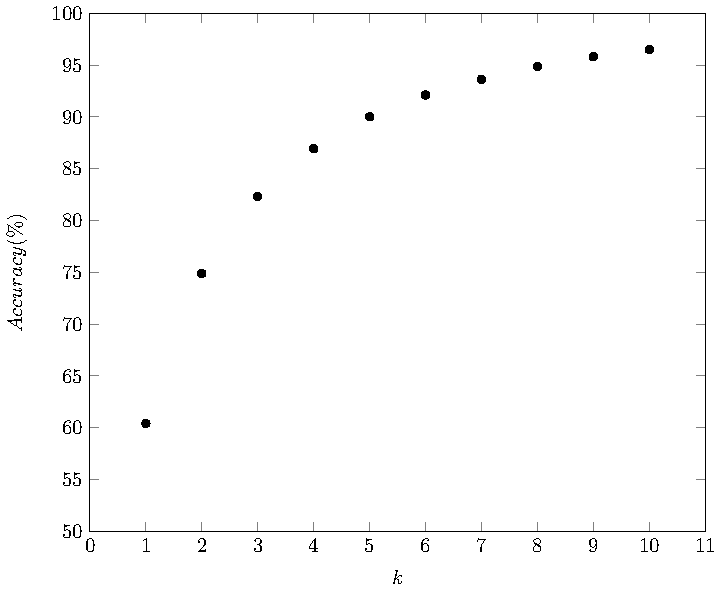
\includegraphics[width=0.7\linewidth]{topk.pdf}
\captionof{figure}{\color{Green} Prediction accuracies of the policy net.}
\end{center}
\end{minipage}%\vspace{1cm}
\begin{minipage}{0.3\linewidth}
{ \color{Green}
MSE of value net:
\begin{itemize}
\item Train: 0.067
\item Test: 0.083
\end{itemize}
}
\vspace{8cm}
\end{minipage}

\subsection*{Empirical performance}
Using fixed widening factor for all expanding nodes, could FDFPN perform better by replacing its move
ordering function from Resistance to policy net?
\begin{center}\vspace{1cm}
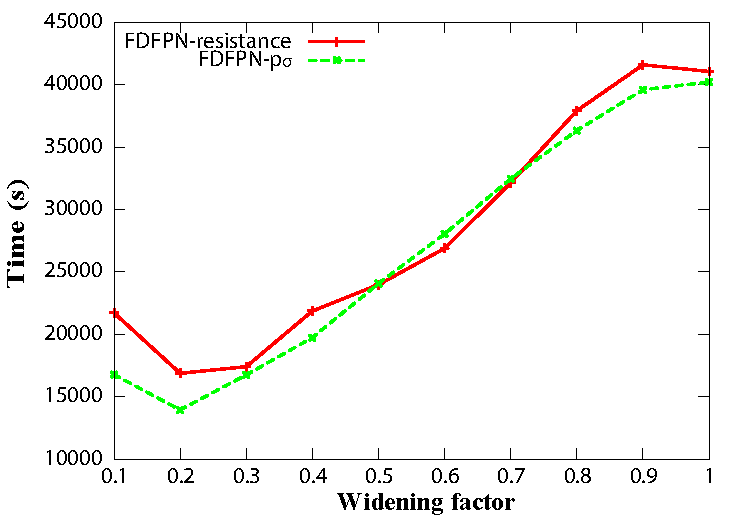
\includegraphics[width=0.8\linewidth]{mycompare.pdf}
\captionof{figure}{\color{Green} Policy neural net is better at ranking strong moves than Resistance.}
\end{center}\vspace{1cm}
\begin{itemize}
\item Policy net is better at small winder factor.
\item Widening factor is close to 1, both recede to normal DFPN.
\end{itemize}

\subsection*{Solving all $8\times 8$ openings}

Improvement of FDFPN with both policy and value nets (compared to original FDFPN):
\begin{itemize}
\item \#expansion: 46.7\%
\item \#time: 40\% \footnote{Due to the update of Tensorflow, the program gets a bit faster}
\end{itemize}

\subsection*{Further investigation of the value net}
In the discovered solution graph, for each node,
compare the estimated value with ground truth.

A simple classifier can be defined:

$$f(s) = \begin{cases}
1, \mbox{ if } v_\theta(s) > 0 \\
0, \mbox{ if } v_\theta(s) \leq 0  
\end{cases}
$$


\textbf{Error rate} of $f$: $14.3\%$. 

%----------------------------------------------------------------------------------------
%	CONCLUSIONS
%----------------------------------------------------------------------------------------

\color{SaddleBrown} % SaddleBrown color for the conclusions to make them stand out

\section*{Conclusions}
The better performance of FDFPN-CNN is due to two reasons:

\begin{enumerate}
\item Better move selection using policy net,
\item Creating ``artificial'' non-uniform branching factor with value net.
\end{enumerate}

FDFPN-CNN shows that incorporating learnt knowledge to proof number search is possible. 
It is a promising direction since it is easy to generate \textbf{training data} from strong players.
 
\color{Black} % Set the color back to DarkSlateGray for the rest of the content

%----------------------------------------------------------------------------------------
%	FORTHCOMING RESEARCH
%----------------------------------------------------------------------------------------

\section*{Forthcoming Research}

Further improvement is quite possible. 
\begin{enumerate}
	\item Better neural network design. Perhaps residual neural net. More regularization...
	\item Dealing with the imperfectness of the training data. 
	\item Exploiting AND/OR structure to improve the value estimation accuracy. 
	\item Modify the calculation/initialization of proof and disproof number with value net.
    \item Or define a new search paradigm with neural nets other than proof number search.
\end{enumerate}

 %----------------------------------------------------------------------------------------
%	REFERENCES
%----------------------------------------------------------------------------------------

%\nocite{*} % Print all references regardless of whether they were cited in the poster or not
%\bibliographystyle{plain} % Plain referencing style
%\bibliography{sample} % Use the example bibliography file sample.bib

%----------------------------------------------------------------------------------------

\end{multicols}
\end{document}
